\documentclass{article}
\usepackage[utf8]{inputenc}
\usepackage[T1]{fontenc}
\usepackage[german]{babel}
\usepackage{blindtext}
\usepackage{graphicx}
\usepackage[colorlinks=true,linkcolor=black]{hyperref}
\usepackage[affil-it]{authblk}
\newcommand*{\quelle}{
  \footnotesize Quelle:
} 
\title{Dokumentation HappyWriter (Online-Shop)\\ Modul 151\\ Hohlstrasse 535 \\ 8048 Zürich}
\date{09.07.2018}
\author{Lars Gächter
\thanks{Elektronische Adresse: \texttt{lars.gaechter1998@hotmail.com}; Korrespondierender Autor}}
\affil{Stiftung Wirtschaftsinformatikschule Schweiz WISS}
\begin{document}
\maketitle
\clearpage
\tableofcontents
\clearpage 
\begin{abstract}
In diesem Pojekt handelt es sich um eine Webapplikation welche ein Online-Shop ist, in welcher die Speicherung und die Verwaltung von Daten mit einer Datenbank unterstützt ist.
Es ist ein Java Projekt welches mit dem Framework WebObjects und Wonder umgesetzt ist.
\end{abstract}
\section{Einleitung}
\section{Anforderungen und Betriebsanleitung}
\subsection{Anforderungen}
Komplette WOnder Umgebung installiert\\
Eclipse\\
Java 8
\subsection{Getestete Funktionsfähigkeit}
Software\\
JRE JDK 1.8.0 171\\
WebObjects version 5.4.3\\
WOLips WebObjects 5.1 Eclipse Plugin\\
Java 8\\
MySQL und MariaDB\\
Eclipse IDE for Java Developers\\
Version: Oxygen.3a Release (4.7.3a)\\
Build id: 20180405-1200\\
Edition: Windows 10 Home\\
Version: 1803\\
OS Build 17134.137
\subsection{Betriebsanleitung mit Hilfestellung}
Java Projekt importieren\\
Kopieren und entpacken Sie den Ordner happywritter in den workspace Ordner von Ihrem Eclipse.
Starten Sie Eclipse und binden Sie das den entpackten Ordner happywritter als ein bereits bestehendes Projekt ein.\\
Datenbank\\
Starte Sie Ihre MariaDB oder MySQL Datenbank und führen Sie das sql mit Ihrem root Benutzer aus, welches sich im Ordner sql im obersten Verzeicnis welches sich im happywritter Ordner befindet.
\section{Datenbankmodellierung}
\subsection{ER-Modell}
\begin{figure}[h]
\begin{center}
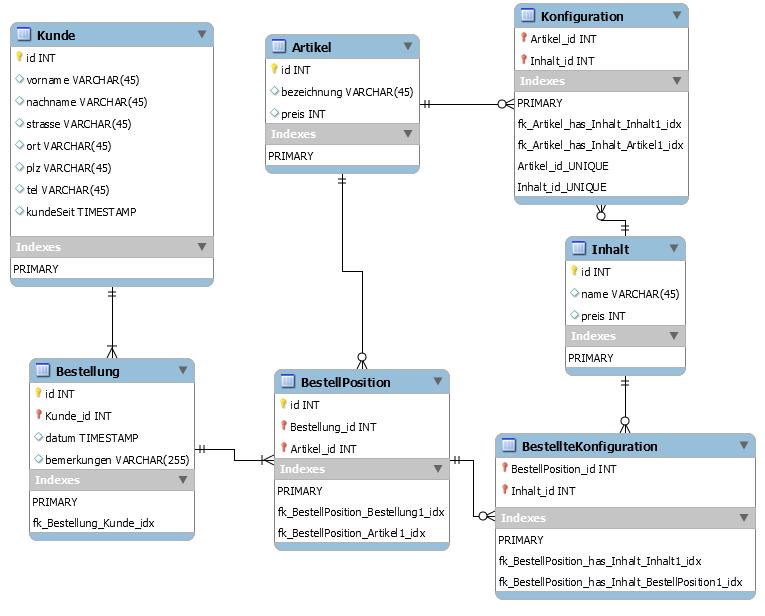
\includegraphics[width=0.7\textwidth]{res/erd.png}
\caption{ER-Modell}
\label{er-modell}
\end{center}
\end{figure}
\subsection{Entitäten und Attribute}
{\large Kunde}
Ist eine Person mit Vorname, Nachname, Strasse, Ort, Postleitzahl, Telefonnummer und Registrierdatum im System\\
\\
{\large Bestellung}\\
Datum der Bestellung, Bemerkung zur Bestellung\\
\\
{\large Bestell Position}\\
Trägt kein Attribut, ist für die Zuweisung eines Artikels für die Bestellung zuständig\\
\\
{\large Artikel}\\
Hat eine Bezeichnung und einen Preis\\
\\
{\large Inahlt}\\
Hat einen Namen und einen Preis 
\subsection{Beziehungen}
Speziell ist zu beachten, dass ein Artikel nicht in einer Bestell Position enthalten sein muss, um ein Artikel zu sein.\\
So ist auch eine Bestell Position immer noch eine Entität auch wenn diese in keiner Bestellkonfiguration vorkommt.\\
Damit aber Einträge in Bestell Position, Konfiguration und Bestellte Konfiguration valide sind, dürfen keine Referenzen nicht zugewiesen (null) sein.\\
\\
{\large Konfiguration}\\
Administrator vom Webshop kann bestimmen und strikt vorgeben, welche Beziehungen von Artikel und Inhalte eingegangen werden dürfen.\\
Damit bei der Konfiguration keine Duplikate entstehen würde sich ein Unique Index als nützlich erweisen.\\ 
\\
{\large Bestellte Konfiguration}\\
Der Kunde ist auch in der Lage Artikel mit Inhalte zu kombinieren, ist jedoch von den Konfigurationen des Administrators eingeschränkt.\\
Wenn der Kunde zu einem Artikel einen Inhalt mehrmals enthalten haben möchte, fehlt hier die die bestimmbare Anzahl von Inhalte, dies müsste redundante Einträge in der Bestellen Konfiguration erlauben.\\
\subsection{Abhängigkeiten}
Nicht abhängig sind Kunde, Artikel und Inhalt, welche unabhängig anderer Existenzen sind.
Für eine Konfiguration des Administrators benötigt es mindestens einen Artikel oder einen Inhalt, da diese null sein dürfen.\\
Für eine Bestellte Konfiguration des Kunden benötigt es mindestens eine Bestell Position oder einen Inhalt, da diese null sein dürfen.\\
Für eine Bestellung wird mindestens ein Kunde benötigt, welcher diese aufgegeben hat.\\
Eine Bestell Position benötigt und gehört genau zu einer Bestellung, kann aber ohne einen Artikel existieren, somit sind leere Bestellungen möglich.\\
Pro Bestell Position sind maximal ein Artikel möglich, so können auch existierende Artikel nicht in einer Bestell Position vorhanden sein, da kein Kunde diesen Artikel bisher bestellt hat.\\
\section{Klassendiagramm und Objekte}
\subsection{Klassendiagramm}
\begin{figure}[h]
\begin{center}
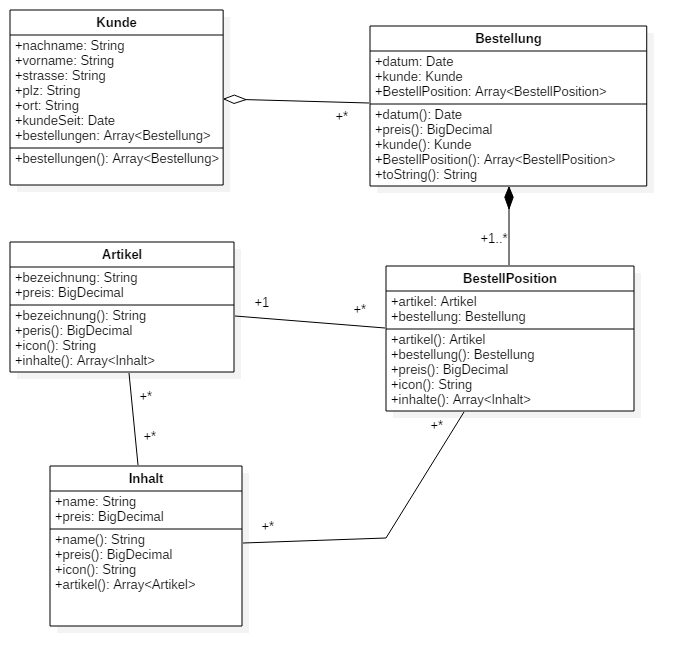
\includegraphics[width=0.7\textwidth]{res/uml.png}
\caption{Klassendiagramm}
\label{klassendiagramm}
\end{center}
\end{figure}
\subsection{Objekte und Verhalten}
Auf Eigenschaften von den Objekten gehe ich nicht mehr weiter ein, da diese schon im Datenbankmodell schon erwähnt wurden.\\
Es stellt sich mehr die Frage, wie kennen sich die Objekte gegenseitig und was ist Ihr verhalten und dabei nicht an Datenbank zu denken war und ist für mich immer noch schwierig.
Eine Datenbank speichert die Daten in einer Struktur, so dass diese möglichst effizient abgefragt und Redundanzen vermeidend gespeichert werden können wenn möglich.
Ein Objekt selbst sagt nicht, ich bin ein Objekt einer Tabelle einer Datenbank sondern ein Objekt einer Klasse und habe Verhalten, Eigenschaften und kenne übergreifend andere Objekte.
In der Datenbank ist es interessant diese Eingeschalten von einem Objekt zu speichern, wie sich dieses verhaltet ist der Datenbank völlig egal, was sind die Beziehungen von Daten ist gefragt.\\
\\
Verhalten der realitätsnahen Objekte, so wie jeder sie kennt.\\
Jedes Objekt kennt sich selbst, aber nicht die anderen oder möchte andere höflich fragen, wenn es etwas von jemand anderen (Objekt) etwas möchte.
Das Kunde Objekt möchte gerne etwas im Online-Shop bestellen, somit gibt der Kunde seine Eigenschaften an, welche von Ihm verlangt werden.
Ein Bestellung Objekt möchte wissen, von welchem Kunden Objekt diese Bestellung angefordert wurde und wie viele Bestellpositionen für alle Artikel nötig sind.
Das Beziehungsobjekt Bestellte Konfiguration kennt das Beziehungsobjekt Konfiguration nicht, kein Problem das Objekt Inhalt steht in Kontakt zu beiden Beziehungsobjekten
und ist daher die Schnittstelle um zu vermitteln welche Beziehungen das Objekt Kunde Bestellte Konfiguration überhaupt anfordern darf.
Indirekt sind alle Objekte wie Artikel, Inhalte mit den zwei Beziehungen dazwischen miteinander verknüpft und jeder weiss von einem anderen Objekt etwas.
Da jedes Objekt Bestellposition nur ein Objekt Artikel sich merken kann, müssen pro Objekt Bestellung mehrere Objekt Bestellposition vermerkt werden können.
Die tatsächliche Objekte Inhalt welche das Kunde Objekt angefordert hat, werden im Objekt Bestellte Konfiguration gespeichert und das Objekt Bestellte Konfiguration weiss vom Objekt Bestellposition zu welchem Objekt Artikel alle Objekte Inhalte gehören
, da eine bestellte Konfiguration sich mehrere Inhalte für eine Bestellposition (Bestellposition merkt sich ein Artikel) merken kann.\\
\\
Verhalten von nichts realitätsnahen Objekten, welche oft das System und deren Steuerung sind.\\
Es gibt noch die Session, Applikation und die Datenbank,
welche zu bestimmten Zeitpunkten während des Betriebs sich Daten merken oder mehrere Vorgänge durchlaufen müssen, um Daten vom Benutzer in einer Struktur, welche die Objekte in sich tragen zu merken und am Schluss in einer Datenbank zu speichern.
Da es ein Online-Shop ist empfiehlt es sich die zu speichernden Daten und Interaktionen des Benutzers in einer Session zu speichern, da mehrere Kunden in der Realität eine solche Anfrage auf den Server starten.
Man sollte den Kunden nicht im Online-Shop verwirren und ihm den Kauf und alle nötigen Vorgänge, welche er durchgehen muss, möglichst leicht vorlegen und ihm die nahezu hundert prozentige Kontrolle über sein Interesse an seiner Bestellung geben.
Somit wäre es dem Kunden möglich, unkompliziert einzukaufen und jederzeit Änderungen alter Einstellungen vorzunehmen.
\section{Projektordnerstruktur}
\subsection{Kurzbeschreibung}
Ordnername und Unterordnername
\subsection{Projektordner}
Hauptverzeichnis\\
\path{\happywritter}
\subsection{Resourcen Webapplikation}
Pfad
\path{\WebServerResources}
\subsection{Cascading Style Sheets}
Bootstrap\\
\path{\css}
\subsection{Bilder}
Artikel, Inhalte etc.\\
Pfad
\path{\img}
\subsection{Klassendiagramm Datei}
Pfad
\path{\uml}
\subsection{Datenbank Skript}
Der Skript für die Erstellung der Datenbank mit Testdaten\\
Pfad
\path{\sql}
\subsection{ER-Modell}
Datenbankmodeldiagramm
Pfad
\path{\erd}
\subsection{Dokumentationen}
Alle Dokumentationen sind im Ordner doc zu finden.\\
\path{\doc\javadoc}\\
\path{\doc\eomodeld}\\
\path{\doc\uml}\\
\path{\doc\documentation\output}
\subsection{Quellverzeichnis Java Klassen}
Session\\
Benutzer\\
Application\\
DirectAction\\
Pfad
\path{\Sources\ch\lars\your\app}\\
\\
Klassen Objekte aus dem eomodel generiert\\
Pfad
\path{\Sources\ch\lars\your\app\eomodel}\\
\\
Klassen für die Webkomponenten\\
Pfad
\path{\Sources\ch\lars\your\app\components}\\
\\
\subsection{EOModel}
Pfad
\path{\Resources}
\subsection{mysql Connector jar}
Pfad
\path{\Libraries}
\subsection{Komponenten}
Pfad
\path{\Components}
\subsection{Build der Klassen}
Pfad
\path{\bin}
\subsection{Build der WO Komponenten}
Pfad
\path{\build}
\section{Benutzungsanleitung mit Hilfestellung}
Wenn die Webapplikation und die Datenbank im Hintergrund gestartet sind und Sie sich auch auf localhost:port im Browser begeben haben,
wird Sie eine Startseite erwarten, welche zum Kunde Webshop und Administrator verzweigt.
Es gibt zur Navigation mit Bttons im Webshop noch etwas wichtiges zu beachten.
Es gibt einen Zurück Button welcher nichts speichert und einen Schritt zurückgeht.
Es gibt einen Bestätigungsbutton welcher die Daten Speichert und auch wenn die Angaben des Kunden nicht wollständig waren.
Der Abbruch Button ist mit Vorsicht zu geniessen, da dieser Ihre Sitzung beendet und alle Ihre Angaben komplett vergisst und Sie an die Startseite zurückleitet.
\subsection{Administrator Login}
Drücken Sie auf den Button welcher Sie zum Administrator Login weiterleitet.
Sie haben immernoch die Wahl eins zurückzugehen mit dem zurück Button.
Sie können sich mit Benutzername admin und Passwort klapp42stuhl als Administrator anmelden.
Angemedet sieht man alle Daten welche momentan in der Datenbank gespeichert sind, wenn aber keine Daten vorhanden sind, gibt es auch nichts anzuzeigen.
Sie können neue Inhalte hinzufügen in dem Sie einen Namen und den Preis für den Inhalt eingeben und mit erstellen bestätigen.
Die Zuweisung von Artikel und Inhalt hat teilweise zu problemen geführt und ist darum nicht mehr in der Admin Seite verfügbar.
Sie können jedoch alle Daten aller Tabellen in der Datenbank sehen.
Die mehrfach zu mehrfach Beziehungen können etwas verwirrend eindrücklich erscheinen.
Um diese besser lesen zu können, empfihlt es sich die Fremdschlüssel und Primärschlüssel aus anderen Tabellen miteinander zu vergleichen.
Wenn Sie mit Ihrer Administration fertig sind, können Sie den Admin Benutzer abmelden.
\subsection{Kunde Webshop}
Drücken Sie auf den Button welcher Sie zum Kunde Webshop weiterleitet.
Nun sollten zwei Bilder oben erscheinen, welche alle Artikel vom Webshop darstellen.
Ich möchte Sie noch darauf aufmerksam machen das pro Bestellung nur eine Bestellposition und somit auch nur ein Artikel pro Bestellung möglich ist.
Sie können auf eins klicken und Sie werden an eine Detail ansicht weitergleitet, Sie können keine Inhalte Ihrem Produkt zuweisen was die bestellte Konfiguration sonst erlauben würde.
Sie sehen den Namen, Preis und ein einzelnes Bild vom Artikel.
Sie können, den ausgwählten Artikel bestätigen oder nicht bestätigen oder Ihren Shopbesuch komplett abbrechen mit den drei Buttons unten.
Wenn Sie Ihren gewünschten Artikel bestätigt haben, können Sie nochmals den Preis sehen und das Total ist gleich gross wie ein Artikel kostet.
Da beide Artikel die genau gleiche Speicherung in der Sitzung beanspruchen ist es sogar möglich, dass sich beim bestätigen des anderen Artikles sich gegenseitig darin überschrieben oder sich selbst oder gegenseitig entfernen können.
Es wird keine Liste aus Pestellpositionen-Artikel und bestellte Inhalte im Hintergrund erzeugt.
Neu müsste Ihnen auch der Checkout Button nach der Bestätigung eines Artikels aufgefallen sein.
Wenn Sie auf Checkout drücken können Sie ihre Kundendaten angeben und Sie haben nach wie vor die drei bereits erwähnten Optionen.
Wenn Sie einfach zurück gehen wird nichts gespeichert, falls Sie aber auf bestätigen drücken werden Ihre Angaben in der Sitzung gespeichert auch wenn das Formular nicht valide ausgefüllt wurde.
Zur Validierung, es wird kein leeres Feld und kein Feld mit 50 Stellenlänge akzeptiert.
Wenn Sie das Formular valide ausgefüllt und bestätigt haben, wedren Sie an eine Bestätigungsseite Ihrer Bestellung weitergeleitet.
Hier haben Sie immernoch die drei Optionen, SIe können immernoch ein bis paar mal zurückgehen und alles nochmal anpassen falls Sie es sich anders überlegt haben oder Sie bestätigen Ihren Kauf.
Wenn Sie Ihren Kauf mit bestätigen abgeschlossen haben, wedren Sie an eine Danke Seite für Ihren Einkauf weitergeleitet und Ihre Sitzung ist somit beendet.
Sie haben immernoch die Möglichkeit von hier aus zur Startseite zu gelangen.
\section{Quellenangabe}
Bootstrap Sketchy Theme\\
\quelle\url{https://github.com/thomaspark/bootswatch}\\
mysql-workbench-plugin-doc-generating\\
\quelle\url{https://github.com/letrunghieu/mysql-workbench-plugin-doc-generating}\\
EOModelDoc\\
\quelle\url{https://wiki.wocommunity.org/display/WOL/EOModelDoc}\\
GitHub Logo in der Applikation\\
\path{\happywritter\WebServerResources\img\GitHub-Mark-32px.png}\\
\quelle\url{https://github.com/logos}\\
\end{document}\\